
The method proposed here is built around two processes, each of which may be implemented in a number of ways (including through manual processing):

\begin{enumerate}
    \item Corpus profiling, which produces a metadata-only description of the corpus as a multivariate distribution;
    \item Targeted retrieval, attempting to produce a corpus with the same distribution.
\end{enumerate}

The latter of these may be accomplished most easily by a process of bootstrapping: using Monte Carlo methods to sample from a conditional distribution.  These samples can then be sought a number of ways, such as manual (or crowdsourced) selection of documents, or use of existing search tools.

\subsection{Profiling}
The process of constructing a corpus description is outlined in~\ref{fig:rebuilding:profiling}.  This may be started either from a seed corpus, or from direct user design.

\begin{figure}[h]
    \centering
    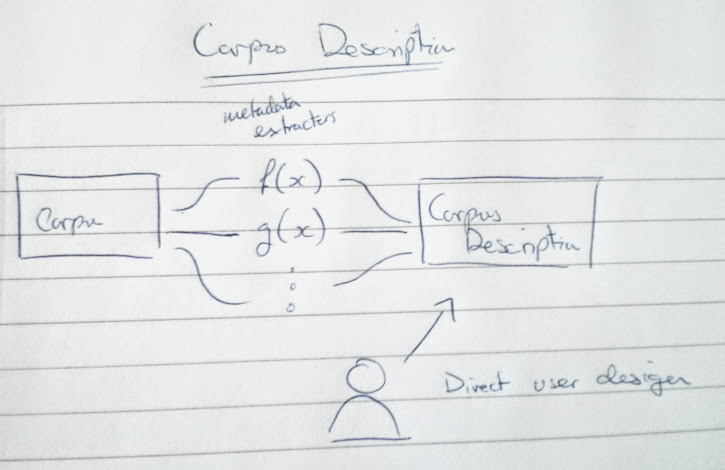
\includegraphics[width=0.8\textwidth]{rebuilding/profiling}
    \caption{Creation of a corpus description}
    \label{fig:rebuilding:profiling}
\end{figure}


For direct use, the user would specify their salient dimensions, and the distribution for each.  This is essentially a description of the sampling policy---where variables are discrete and nominal (such as genre labels), this would take the form of a table with desired proportions against each.  Where variables are continuous, a probability density function is defined.  Note that this method does not, without prohibitive complexity, allow for specification of interactions between variables, leaving it unable to represent, for example, differing genres within spoken and written portions of a corpus\td{c,o,m,m,a,s}\td{return to this and comment on it later}.

Profiling through the use of a `seed' corpus begins with specifications of the salient dimensions, the data for which are then read from the seed (by $f()$ and $g()$ functions in the figure).  As each document is read, the corpus description may contain information not only on marginal distributions for each variable, but also the effects of conditioning on one or more value.

Note that, whichever method is used, this stage is merely a metadata description task.  The corpus description document itself contains no more information than the metadata of the corpus from which is it built---for specifications involving full data on interactions this reduces to a list of points in vector space.  For a corpus designed only by specifying marginal distributions, it constitutes a distribution for each.

Those specifying variables to describe must, as with all sampling, be mindful of potential systematic correlations with variables of interest to any given research question.  The value of the approach presented here is in documentation---it is possible for a researcher to eyeball the variables (and potentially their distributions) and determine whether or not a corpus is correctly conditioned for use inferring about a given variable.  This cannot be said for bootstrapping systems that use internal variables, which seek to copy corpus contents at the risk of varying their metadata.

% ---

\subsection{Retrieval}
Retrieval in accordance with the complex distributions specified in a corpus description is challenging in two ways:

\begin{itemize}
    \item Samples must be taken from the corpus description in accordance with a complex empirically-determined distribution;
    \item Any combination of variables sampled from the distribution must then be sought based on its metadata alone.
\end{itemize}

The former of these is difficult because many seed corpora may lack sufficient data to specify their distributions, and because of the high dimensionality of the distributions in question.  These issues may be addressed using techniques such as Gibbs, slice, or rejection sampling.

The sampling of `prototype' documents from the metadata distribution is possible regardless of the manner of its construction (however, those specified as marginal distributions will lack any interactions).  Here we assume a full specification, since this method is the more comprehensive case.

The following subsections will describe these processes in more detail.

\subsubsection{Sampling Metadata}

% \begin{figure}[h]
%     \centering
%     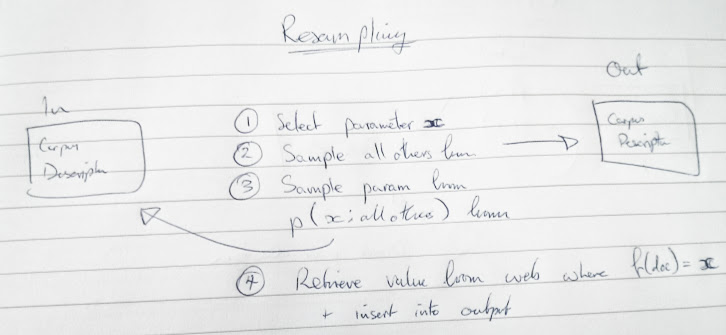
\includegraphics[width=0.8\textwidth]{rebuilding/resampling}
%     \caption{Resampling the corpus using MCMC methods}
%     \label{fig:rebuilding:resampling}
% \end{figure}

Sampling from the seed corpus' profile produces a `prototype' document, which has values of metadata fields that, over time, hold the same distribution as those in the seed corpus.

The process of constructing a new corpus is one of continually producing these `prototypes' conditional on the values of metadata already sampled, and then retrieving texts matching each.

To perform this resampling, we must be able to sample from the distribution of each variable conditional on all of the others, requiring that the corpus description contains information on interactions between values.  As such it is only possible if the original corpus description document contains this information, something that is only practically a product of describing an existing set of documents (as manually filling in the values would be prohibitively expensive).

Two methods were implemented for selection of the prototype, representing two of the most popular use-cases.  

\begin{itemize}
    \item Simple selection from marginals.  This is the best case possible where a corpus lacks interaction information, and follows the joint distribution of the metadata properties across the whole corpus.  Despite its relative simplicity it may be suitable for some corpus designs, and is analogous to the BNC's balancing of spoken corpora \td{check this, cite the page where they describe their balancing}.
    \item Full conditional selection.  This is implemented by recursively selecting a random sequence of metadata types, and then conditioning on a value drawn from the distribution of that type conditional on the values selected for those previous to it.
\end{itemize}

\til{Does this need the algorithm for both here?  It's terribly simple}

It is additionally possible to sample conditioning on fewer variables (yet randomly selecting them each time) in order to emulate the behaviour of a `blocked' Gibbs' sampler\td{cite}.

The former of these, whilst faster and simpler, will fail to take into account any interactions between metadata and is included since it is the only method capable of running on a very simply specified corpus description.  The experiments in this thesis use full conditional selection, as they have the luxury of using a corpus description built from a full seed corpus.


\subsubsection{Seeking the Prototype Document}
\label{sec:rebuilding:design:seekprototype}
The main practical problem of sampling according to the original corpus' distribution is now framed as an information retrieval task---seeking a document that has the same metadata as the one we sampled from seed corpus' profile.  Repeating this `sample and seek' behaviour forms the bootstrapping portion of the method, converging on the input distribution as the output size grows.

This retrieval task is challenging on its own, but errors in performing it have specific ramifications for this sampling process:

\begin{itemizeTitle}
    \item[Dimensionality]As the number of metadata properties in the prototype increases, the search space from which a document must be selected increases exponentially\footnote{Or, strictly, somewhere between linearly and exponentially, if the metadata properties are not truly orthogonal}.  This has severe ramifications for rejection sampling techniques, which become intractable where the ratio of the search space to the area under the target distribution is high.

    \item[Selection of dimensions]Metadata types are selected for research reasons and do not necessarily correspond easily to existing online indexes or retrieval methods.  This means that specifically seeking a document with one value of metadata may be a challenging task.

    \item[Error in selection]In part because of the above point, documents retrieved are unlikely to be a perfect match against the prototype.  Errors in multivariate selection will follow the population distribution conditional on those metadata values being sought: something that will introduce systematic (yet measurable) bias in the dataset\footnote{The one, extremely unlikely, exception to this is if the population distribution happens to be the same as the target.}.
\end{itemizeTitle}

The retrieval of a prototype, then, is limited to approaches that take into account not only the value of a metadata property to be sought, but also the nature of the source (in this case the internet) and any interactions that are likely to expand the search space to intractable proportions.  It should also, of course, minimise error in selection.


\begin{figure}[h]
    \centering
    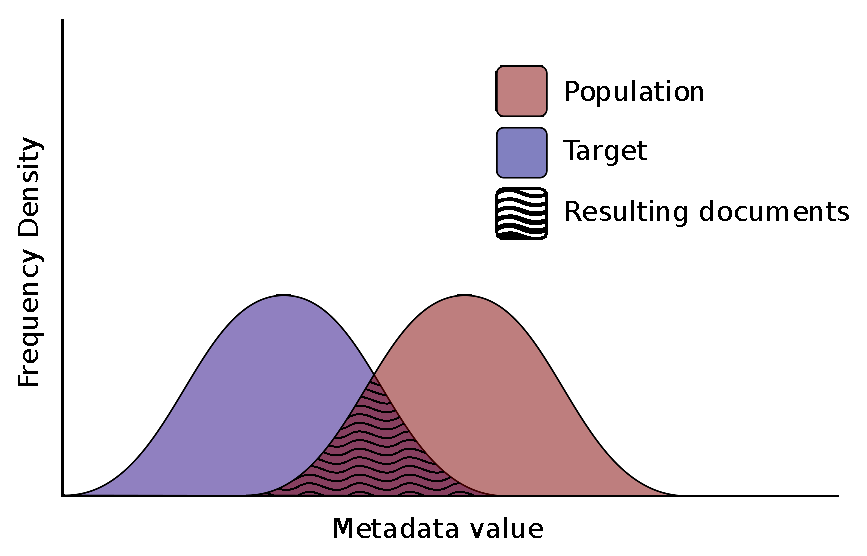
\includegraphics[width=0.8\textwidth]{rebuilding/population-bias}
    \caption{The influence of a biased population distribution on metadata selection}
    \label{fig:rebuilding:population-bias}
\end{figure}


In such a case that the retrieved document is a perfect match to the prototype, the output set of documents will converge to the target distribution.  If it is imperfect but randomly so, there will be an increase in variance in the output distribution.  If it is imperfect and the population is not a superset of the input distribution (or, in the worst case, does not overlap even slightly with the target), then the results will converge to a distribution with bias following the population distribution.  In terms of Figure~\ref{fig:rebuilding:population-bias}, we rely on the blue distribution falling entirely within the red one.


It is unlikely that the search space for documents in the population will \textsl{always} encompass the range of the input corpus.  In such cases the population will bias the output corpus, something that is also evident in existing bootstrapping tools such as BootCaT~\cite{baroni2004bootcat}.  The rejection sampling approach used here, however, makes it possible to measure the difference between the document selected for output and the prototype; providing a measure of error for the sampling method in a manner inaccessible to conventional bootstrapping.  This is essentially controlling for population and search engine effects that are otherwise conflated with the distribution of the input data.

%The last of these is the product of an attempt to do something fundamentally impossible: the design of the system is such that this bias is measurable (and may thus be seen to be above some subjective threshold) rather than that it is eliminated for every scenario.  This bias is also evident in existing bootstrapping tools such as BootCaT~\cite{baroni2004bootcat}, however, they seek a looser form of coupling between input and output distributions so this bias often goes un-noticed (or, perhaps, desired\footnote{The comparison of distribution of seed terms to resultant type frequencies yields information about the search method and population, though these are conflated in the process}).

Instead of sampling a corpus \textsl{of} the web, we are sampling one \textsl{from} it, on assumption that the web is already a poorly-indexed supercorpus of documents that are diverse enough to satisfy the majority of research questions.  In terms of Figure~\ref{fig:rebuilding:population-bias}, we assume that the distribution in red has a very high variance (not just in one dimension as illustrated, but also in interaction with other metadata).  Clearly, the case in which this assumption is least strong is the replication of web corpora, and it is perhaps most strong for speech or other particularly specialist sources such as medical notes.

% ---

There are multiple possible approaches to this retrieval task, which mirror the web corpus building approaches of searching and sorting.  Each type of metadata may use one or many of these, depending on their relationship to the structure of the web.  They are listed here in descending order of `direct applied expert opinion': the first item in the list relatively dispassionately seeks similarity, and the last uses human judgement directly to identify documents.



\paragraph{i. Searching}
\label{sec:rebuilding:design:searching}
Using similar methods to BootCaT and other seed-based corpora, it is possible to identify documents conforming to certain metadata values by using a search engine.  This encounters minor difficulties in that it is often necessary to transform an ostensive definition (e.g.\ the domain from which a text is drawn) into an intensional one (i.e.\ some keywords or other features typifying the domain) in order to fit the format desired by search engines.

If the method detailed here is used only for metadata types which are retrieved by example (the intensional definition above), then this technique for document-seeking is functionally identical to BootCaT's approach.



\paragraph{ii. Directed Crawling}
Another technique widely used in existing tools is crawling.  When downloading documents using a spider, it is common to identify the next set of links (the `fringe') and then select from the fringe using a suitability metric.

The problem of directing a spider is then one of relating the features visible about a link (link text, url features, position in text, etc.) to the value of a document that will be gathered.  This will often involve similar issues to the searching method: it is necessary to examine document content and compare it to some ideal of each metadata value in order to form the link.

Many spiders currently focus on document `goodness' by simple definitions of information content or URL features~\cite{schafer2014focused,ferraresi2008introducing,belikov2013big}---these produce samples that are designed to approach simple random samples (SRS) in order to approximate the population of sites over which they run whilst exploiting the hyperlinked structure of the web.  The approach required to deliberately skew this search is arguably an easier problem: a spider may follow rules based on keywords or site features, rather than modelling the content of documents in great detail.

The starting point of each spider may itself be determined by using a search engine.  This is common practice, used to direct spiders to relevant starting points, however, the ratio of crawling/searching used for any given selection may greatly change the output.



\paragraph{iii. Existing Indices}
The use of existing indices for certain types of metadata is a main technique used in conventional corpus construction.  Online, however, this avenue is often neglected (with the notable exception of WebCorp~\cite{renouf2003webcorp} and Barbaresi's examination of indices as seed URL sources~\cite{barbaresi2014finding}) despite the existence of many subject-specific indices and general-purpose manually-curated web directories.

By aligning the taxonomies used in metadata to those in an existing web directory, it becomes possible to use the contents of the directory to access documents authoritatively categorised by humans (or to start crawling from these).

This method is subject to errors regarding the age of content on web directories (the popularity of which is waning in favour of search engine technology), as well as those introduced by human categorisers whose aims may not be aligned to the definitions required for a given research question.  Additionally, the granularity of each category is fixed and cannot reasonably be changed.

Nonetheless, such an approach is close to that used in conventional corpora and is easily defended, providing that the directory is well trusted.%  It should be noted that some web directories are already used by search engine operators to augment their taxonomies.
\til{Note that `best of the web' has a specific blog directory and is used by search engines}

\paragraph{iv. Manual Selection}
Crowdsourcing services offer a cheap mechanism for retrieving documents by requesting that humans manually seek a document fitting the prototype metadata.  This method has severe volume and speed limitations not present in the others, however, the accuracy of a human search is likely to be far greater, minimising overdispersion in the output set.

Where a corpus must be duplicated as accurately as possible (yet there is less importance placed on scale or speed of rebuilding), this is most likely a good choice for almost all metadata properties.

The major disadvantage of this method is that the speed of lookup is greatly reduced, bringing the corpus building process closer to that used by a conventional corpus.  The main difference here is that the weight of expertise required to select documents is handed off to those constructing the corpus definition, rather than those searching the indices.







\subsubsection{Candidate Selection}
% The process of running heuristics will return a set of candidate documents, each of which will be returned under the condition that it satisfies the metadata property that each heuristic is designed for.  The size of this set is dependent on the probability of error, and is discussed below in Section~\ref{sec:rebuilding:design:minerr}.

Since each retrieved document may be missing metadata in some dimensions, it is necessary to infer the values for these from the document itself.  This process may use external variables such as HTTP headers/meta-tags in the header of the document, or internal ones that are assessed using some measure unrelated to the variables of interest to those constructing the corpus.  This process is performed by a number of heuristics, and may be thought of as an inverse function to the profile generating functions shown in Figure~\ref{fig:rebuilding:profiling}.

Documents may be ranked by similarity in vector space only after normalising each metadata distance metric (otherwise, distance metrics liable to output large numbers would be apportioned a larger importance in overall fit).  This method also allows imposition of weights to specify which dimensions must fit more accurately.


\subsubsection{Iterating to Minimise Error}
\label{sec:rebuilding:design:minerr}
It is necessary to iterate an arbitrary number of times to retrieve a full corpus.  If each prototype document is matched closely, a simple repetition of the above will return a corpus that converges to the desired distribution, however, as mentioned in Section~\ref{sec:rebuilding:design:seekprototype}, this approach may incorporate bias from the population.

There are two possible approaches to working with biased populations:

\begin{itemizeTitle}
    \item[Feedback from output to target distribution] Adjust the target distribution to reduce the probability for those documents already selected.
    \item[Rejection sampling]  Select a large number of candidate documents and then identify the document (or subset of documents) that best fits the prototype
\end{itemizeTitle}

The former of these approaches may seem ideal, however, it will only be effective if sufficient documents have already been selected for each conditional distribution, and if the population distribution is only slightly biased.  It will also slow down the seeking stage of each document and, in the event that the population yields no perfect documents, stop it completely.  It is a stricter and more reliable approach, but also vastly reduces the practicality of any system using it.

Variations on this theme form the basis of many MCMC methods, particularly Metropolis-Hastings.  MCMC algorithms are generally used where it is difficult to estimate marginals, however, this is not the case for our corpus data.

\til{Check that there isn't some way these can be used\ldots [DL]}

The latter, rejection sampling, is much more viable, as the clustered and hyperlinked nature of the internet makes retrieval of many similar documents only slightly more difficult than retrieval of just one.

The (hyper-)volume of the search space increases greatly as dimensions are added.  This is largely mitigated by the directed document hunting approach above, which seeks to minimise the distance between each dimension's sampling distribution and the target.  Simply, the better the heuristics are (measured in terms of precision/recall), the more tractable any selection is and the fewer documents that need selecting.  The number of documents that needs selecting is proportional to the ratio of the areas under the joint distributions of the PDF of the heuristics' selections over those of the target distribution:

$$
numdocs \propto \int{\prod{heuristics}} / \int{\prod{target}}
$$

This presumes that each of the dimensions selected is entirely orthogonal, but serves to illustrate the curse of dimensionality that applies to the search space.

Where a target is defined in terms only of its marginals (as is likely when constructing a corpus from scratch), the interactions observed will be defined by the source population (in this case online), and the sample will exhibit conditional distributions that are peculiar to the internet regardless of its marginal distributions.  This approach relaxes the original sampling criteria applied to the seed corpus too, making replication far simpler at the expense of any best-effort approach to minimising bias across multiple dimensions.

As the population distribution for each dimension is unknown (especially if one considers interactions), it is impossible to know to what degree it is being undersampled.  This is another source of bias, however, it is one that is clearly labelled as such: those using a heuristic would do well to know its theoretical underpinnings and the methods it uses to select data (just as any corpus user should read the manual).

The main benefit of rejection sampling is that we are able to degrade the performance of the algorithm gracefully.  If, having sampled $n$ documents, we wish to relax the conditions of a match with the prototype, this will have only a minor effect on the corpus (increasing its variance and applying a small bias in the direction of the difference between the population and target modes).  

The degree to (and conditions under) which this relaxation occurs must be determined according to the particular demands of the application for which a sample is being built.



\subsection{Measuring Fit}
A system built with contingency for accepting certain levels of error is of very little use without some method for measuring it in operationalisable terms. A number of properties of the system are measurable, each yielding information that is useful under different circumstances:


\paragraph{Heuristic Quality}
The quality of each heuristic may be measured according to its ability to return documents satisfying the one metadata value it is seeking.  This may be expressed in terms of precision and recall, or an aggregate thereof such as an F-score.

The choice of evaluation metric will vary according to the type of metadata and its availability online.  Heuristics operating in particularly large search spaces (such as those primarily using search engines) will desire a greater weight on precision, whereas those seeking rare (online) data will favour recall.  Since heuristics are, ideally, already the results of well-established methods in linguistics, this score and its desirable range should be established empirically prior to use.

The F score may also be generated only for the best documents returned, providing a score for the whole `batch' of documents returned by a heuristic.  This measure is likely to be more representative of stateful heuristics (i.e.\ those that crawl), however, it conflates the statistics used for measuring document similarity with those used to retrieve them.

Ideally, heuristics form pluggable, reliable modules with known degrees of error that may be ignored when using the method as a source of linguistic data.  The degree to which this applies is defined by how well each is aligned with a source of data: Keyword-based heuristics, for example, are well aligned with the search systems of search engines, but poorly aligned with the strengths and weaknesses of humans seeking a document type.

The value a heuristic yields is a trade-off between how closely it describes the document and how accurately it is possible to retrieve a document from the source. \td{perhaps remove, poorly worded}


\paragraph{Document Distance}
It is necessary to identify differences between documents' metadata values both in order to select them from the set returned by each heuristic and to identify overall deviance from the target distribution.  The former is computed after documents have been retrieved by a search method but prior to their selection; the latter after selection.

Boolean selection criteria (are the metadata in this document equal to the prototype) offer a way to guarantee convergence to the target distribution.  They are an ideal case which will be tractable in only certain circumstances.

Relaxing the similarity requirement requires a finer-grained distance metric for each metadata value.  The distance for each candidate document may then be measured and a `best fit' selection made.  Alternatively, upper bounds may be set on suitable distances from the prototype for each metadata type, leading to selection of all documents which satisfy those criteria.

Having selected candidate documents using heuristics, it is possible to estimate and then sum the distance each has to its intended value from the prototype.  The sum of squares of each of these will result in the overall error for the final corpus, being analogous to the mean squared error:

$$
MSE = 1/n\sum_{i=1}^{n}\sum_{d \in D}^{d}{(P_i^d - C_i^d)}
$$ 

Where $P_i^d$ is the value of metadata type $d \in D$ of prototype document $i$, with $C$ being the equivalent selected document that was ultimately added to the results set.  $n$ is the number of documents selected.









